% ----------------------------------------------------------
% Aplicação
% ----------------------------------------------------------
\chapter{Aplicação}
\label{chap:aplicacao}

Como esta tese trata do desenvolvimento de um sistema de \textit{software}, não basta apenas
apresentar a metodologia utilizada na sua construção, bem como seus pontos fortes e fracos. É
imprescindível testar o sistema desenvolvido. Para isso, foi desenvolvido um modelo simplificado
\textbf{baseado} em um sistema físico existente, no caso, o reator TRIGA IPR-R1 do CDTN.

A elaboração do modelo levou em consideração os aspectos físicos de um elemento combustível do
reator TRIGA, bem como suas condições de utilização usuais.

O modelo também foi concebido de acordo com as restrições impostas pelos sistemas acoplados utilizados.
O \textit{OpenFOAM}, por se tratar de um sistema mais maduro e com ampla rede de usuários, não impôs
restrições ao problema em termos de tamanho do problema a ser simulado. Entretanto, a versão utilizada,
apresentou um erro (\textit{bug}, no jargão da Ciência da Computação) na implementação da resistência
de contato, o que inviabilizou a simulação do \textit{gap} existente no combustível. Sendo essa a
primeira simplificação necessária em relação ao combustível do reator TRIGA IPR-R1.

No tocante ao \textit{milonga}, as restrições foram maiores. Foram duas as grandes limitações impostas
pelo \textit{milonga} na definição de um modelo complexo. A primeira é relativa a execução de forma
sequencial. Como o \textit{milonga} não é ainda capaz de trabalhar de forma paralela, o tamanho da malha a ser
utilizada fica restrito à memória disponível mas, principalmente, em relação ao tempo de execução. Além disso,
o \textit{milonga} ainda não é capaz de lidar com elementos prismáticos de forma confiável, limitando a
geração da malha por extrusão. Essa limitação não é notável para geometrias com elementos mais homogêneos.
Entretanto, no caso de um combustível do tipo TRIGA, o revestimento tem espessura ordens de grandeza
menor do que o raio do combustível, o que impactou na geração de uma malha mais refinada. A segunda
restrição imposta pelo \textit{milonga}, também em razão de um \textit{bug} está na função de mapeamento
geométrico da malha para estruturas de dados internas. Caso uma região da malha, por exemplo o combustível,
seja formada por células não conectadas, apenas a primeira região é encontrada. Este \textit{bug} tornou
inviável a simulação, dentro da metodologia proposta, de mais de um elemento combustível
\footnote{Durante a execução desta tese, alguns \textit{bugs} encontrados no \textit{milonga} foram corrigidos e
  reportados ao seu autor. Uma das correções acabou com um vazamento em memória que impedia que o \textit{milonga}
  fosse executado mais do que alguns vezes em modo iterativo.}.

Com estas limitações em mente, nas próximas seções será apresentado o modelo utilizado com todas as suas
características bem como os parâmetros utilizados nas simulações neutrônica e termo-hidráulica.

\section{Modelo}

%
% IMPORTANTE
%
% Separo th de neutronica em seções para colocar as seções de choque antes da neutrônica?
% Ou coloco logo as seções de choque antes de tudo?

Nesta seção é descrito o modelo físico e numérico utilizado nos testes do sistema acoplado.

\begin{figure}[htb]
  \caption{Discretização do modelo: regiões e materiais.}
  \centering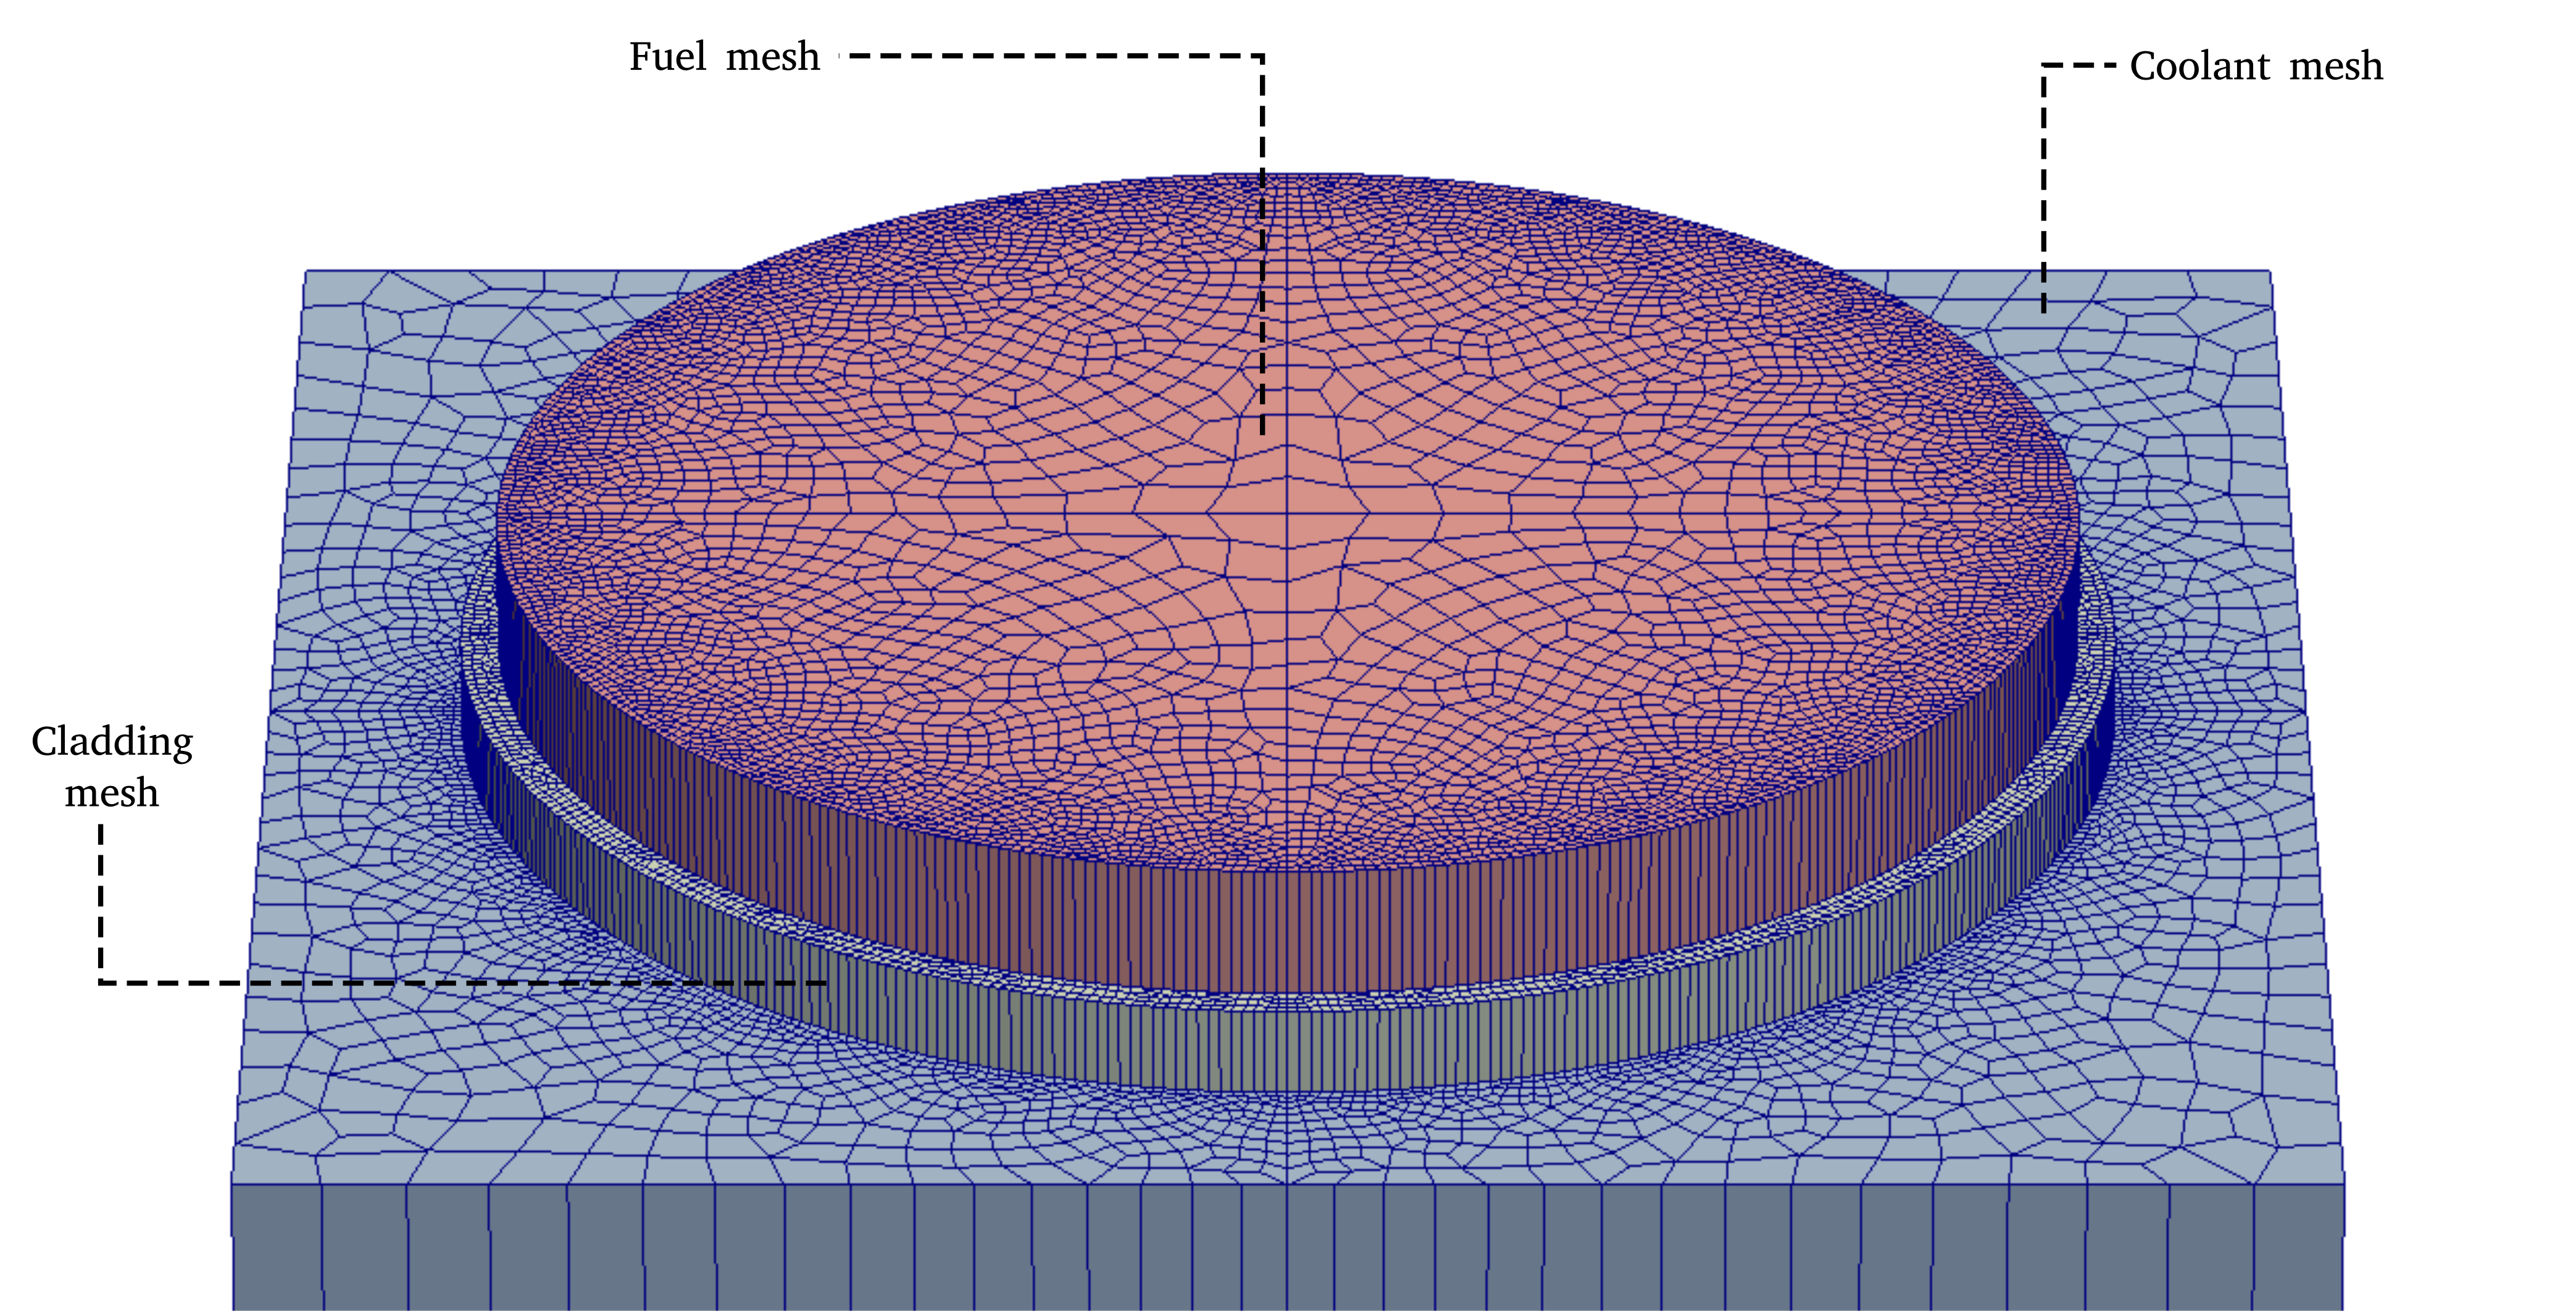
\includegraphics[scale=0.5]{figuras/regioes_edges_com_legenda_ingles.png}
  \label{fig:modelo_exploded}
%  \legend{Fonte: autor}
\end{figure}

\section{Geração de seções de choque}

A fim de verificar o impacto das variações de temperatura calculadas pelo \textit{OpenFOAM} no fluxo
neutrônico e, portanto, na potência volumétrica, foram geradas seções de choque correspondentes
ao modelo utilizado.

para um modelo bidimensional
com propriedades equivalentes ao modelo de malha tridimensional. 

% Não tem figura, ela fez anel anel anel
%Na figura \ref{fig:modelwims}

As seções de choque geradas são usadas como os coeficientes da equação de difusão, como já mencionado.
A tabela \ref{tab:coeff-dif} apresenta o significado dos mnemônicos utilizados pelo \textit{milonga}
bem como a divisão de grupos em energias.

% Tabela para os valores
\begin{table}[htb]
  \caption[Coeficientes da Equação de Difusão.]{Coeficientes da Equação de Difusão.}
  \label{tab:coeff-dif}
  \begin{tabular}{ l | c | r}
  \hline
  \multicolumn{3}{ c }{Coeficientes Mnemônicos} \\
  \hline
  \multirow{4}{*}{Grupo 1: > 0,625 MeV} & Diffusion coefficient & $D1$\\
& Absorption cross-section & $\Sigma A1$\\
& Scattering cross-section & $\Sigma S1.2$\\
  & Neutrons per fission * Fission cross-section & $\nu \Sigma F1$\\
  \hline
\multirow{3}{*}{Grupo 2: < 0,625 MeV} & Diffusion coefficient & $D2$\\
& Absorption cross-section & $\Sigma A2$\\
& Neutrons per fission * Fission cross-section & $\nu \Sigma F2$ \\
\hline
\end{tabular}
\end{table}

Um modelo bidimensional com propriedades equivalentes ao modelo tridimensional a ser simulado
foi definido. Esta equivalência foi garantida mantendo-se a proporção entre material
físsil e moderador em ambos os modelos. Com base nessa proporção,
todos os materiais foram definidos como anéis concêntricos. Geometria definida,
foram geradas seções de choque para quatro diferentes temperaturas, desde
a temperatura ambiente até a temperatura próxima a máxima do combustível do TRIGA IPR-R1 em operação
a $250 kW$ \cite{Veloso2005}. A metodologia utilizada para a geração
das seções de choque considerou as condições do reator TRIGA IPR-R1 no
ano de 2004, sendo utilizado o código WIMSD-5B neste processo \cite{Reis2015}.
As temperaturas utilizadas na geração das seções de choque
e as seções de choque resultantes são apresentadas nas tabelas \ref{tab:temp-fuel},
\ref{tab:temp-cladding} e \ref{tab:temp-coolant} respectivamente para o combustível, revestimento
e moderador.


\begin{table}[htb]
  \caption[Temperaturas para combustível.]{Temperaturas para o combustível}.
  \label{tab:temp-fuel}
  \begin{tabular}{r l l l l}
  \multicolumn{5}{c}{Fuel} \\
  \hline
  Parâmetro & $300K$ & $400K$ & $500K$ & $600K$ \\
  \hline
  $D1$ & 0.0108349 & 0.0108521 & 0.0108489 & 0.010846\\
  $\Sigma A1$ & 0.771135 & 0.783626 & 0.795686 & 0.806567\\
  $\Sigma S1.2$ & 3.3991 & 3.4329 & 3.4264 & 3.4206\\
  $\nu \Sigma F1$ & 0.500982 & 0.500304 & 0.500377 & 0.500441\\
  \hline
  $D2$ & 0.00314942 & 0.0031682 & 0. 0032163 & 0.0032743 \\
  $\Sigma A2$ & 11.0389 & 10.8142 & 10.4004 & 9.90199\\
  $\nu \Sigma F2$ & 20.1943 & 19.7703 & 18.9898 & 18.0499\\
  \hline
\end{tabular}
\end{table}

\begin{table}[htb]
  \caption[Temperaturas para o revestimento.]{Temperaturas para o revestimento}.
  \label{tab:temp-cladding}
  \begin{tabular}{r l l l l}
    \multicolumn{5}{c}{Revestimento} \\
    \hline
    Parâmetro & $300K$ & $396K$ & $403K$ & $410K$ \\
    \hline
    $D1$ & 0.0299644 & 0.0299699 & 0.0299678 & 0.0299659 \\
    $\Sigma A1$ & 0.0288617 & 0.028926 & 0.0289199 & 0.0289143 \\
    $\Sigma S1.2$ & 3.3991 & 3.4329 & 3.4264 & 3.4206\\
    \hline
    $D2$ & 0.0376276 & 0.0376721 & 0.0377696 & 0.0379140\\
    $\Sigma A2$ & 0.874322 & 0.865956 & 0.846858 & 0.818690\\
    \hline
  \end{tabular}
\end{table}

\begin{table}[htb]
  \caption[Temperaturas para o refrigerante.]{Temperaturas para o refrigerante}.
  \label{tab:temp-coolant}
  \begin{tabular}{r l l l l}
    \multicolumn{5}{c}{Moderador} \\
    \hline
    Parâmetro & $300K$ & $308.5K$ & $317K$ & $341K$ \\
    \hline
    $D1$ & 0.0126587 & 0.0126685 & 0.0126696 & 0.0126705\\
    $\Sigma A1$ & 0.0290925 & 0.0292130 & 0.0292018 & 0.0291917\\
    $\Sigma S1.2$ & 3.3991 & 3.4329 & 3.4264 & 3.4206\\
    \hline
    $D2$ & 0.00213616 & 0.0021262 & 0021368 & 0021589\\
    $\Sigma A2$ & 1.42651 & 1.41891 & 1.39505 & 1.35409\\
    \hline
  \end{tabular}
\end{table}

Uma limitação do código WIMSD-5B está na geração de seções de choque de espalhamento
para cada material separadamente. Devido a esta restrição, as seções de choque de
espalhamento foram geradas para uma homogeneização dos materiais em uma única célula,
sendo esta a razão dos valores serem os mesmos para todos os materiais.


%
% IMPORTANTE: Talvez este próximo parágrafo não deva ficar aqui, mas no modelo da neutrônica.
%
As seções de choque obtidas foram então escritas no formato \textit{milonga} como
funções de uma variável dependentes da temperatura. Como o milonga tem informação
das células em relação à malha, a temperatura de cada célula é argumento da
função de uma variável dependente da temperatura. Se a temperatura não está
exatamente tabulada, o \textit{milonga} provê interpolação linear por padrão.

